% Task 3 -- cross-system preconditioning. Compile: pdflatex (x2) in this dir.
\documentclass[aspectratio=169,10pt]{beamer}
\usepackage[T1]{fontenc}\usepackage{lmodern}\usepackage{amsmath,amssymb,bm}
\usepackage{booktabs}\usepackage{graphicx}\graphicspath{{./}}
\definecolor{Struct}{HTML}{1F3A5F}\definecolor{Gray}{HTML}{6E6E6E}\definecolor{Accent}{HTML}{8C2D04}
\usetheme{default}\usefonttheme{professionalfonts}\setbeamertemplate{navigation symbols}{}
\setbeamercolor{structure}{fg=Struct}\setbeamercolor{frametitle}{fg=Struct}
\setbeamerfont{frametitle}{series=\bfseries,size=\large}
\setbeamercolor{block title}{fg=white,bg=Struct}\setbeamercolor{block body}{bg=Struct!6}
\setbeamertemplate{frametitle}{\vskip0.4em\hspace{0.2em}\usebeamerfont{frametitle}\insertframetitle%
  {\ifx\insertframesubtitle\empty\else\\[0.1em]\small\color{Gray}\insertframesubtitle\fi}\par}
\setbeamertemplate{footline}{\hfill\footnotesize\color{Gray}\insertframenumber\,/\,\inserttotalframenumber\hspace{0.4cm}\vspace{3pt}}
\renewcommand{\arraystretch}{1.15}
\begin{document}

\begin{frame}[plain]\vskip1.1cm
{\color{Struct}\large\bfseries Task 3 --- using the earlier system to precondition the later one\par}
\vskip0.4em{\color{Gray} Sys 1 (monodomain) $\to$ Sys 2 (recover $u_e$, singular): implement all options, find the best\par}
\vskip0.8em\hrule height0.4pt\vskip0.5em\footnotesize\texttt{asm\_bug\_demo/cardiac/xsys\_precond.c}
\end{frame}

\begin{frame}{Problem definition --- the exact example}
\framesubtitle{the recover solve driven by the monodomain, every time step}
\[\textbf{Sys 2}:\quad K_{\sigma_i+\sigma_e}\,u_e=-K_{\sigma_i}V_m(t)\qquad(\text{pure Neumann, SINGULAR}).\]
\begin{itemize}\itemsep0.25em\small
  \item As the depolarization wave sweeps the slab, the RHS and $u_e(t)$ vary \textbf{smoothly in time} $\Rightarrow$ the solution sequence lives near a low-dimensional subspace.
  \item Example: Niederer slab $20{\times}7{\times}3$ mm, $h{=}0.5$ (4305 nodes); $\sigma_i{=}(0.17,0.019)$, $\sigma_e{=}(0.62,0.236)$ S/m; a moving sigmoid front (0.6 m/s), 40 consistent (mean-zero) RHS.
  \item Metric: CG iterations per recover solve to $\|r\|/\|b\|<10^{-8}$.
\end{itemize}
\end{frame}

\begin{frame}{All cross-system options, and the best}
\begin{center}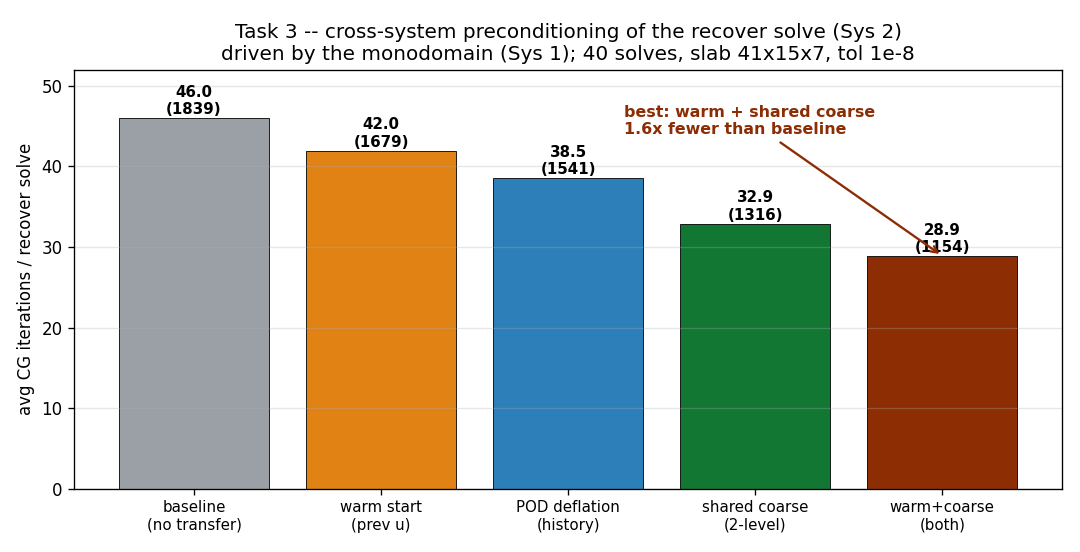
\includegraphics[width=0.78\textwidth]{fig_xsys}\end{center}
\vskip-0.25em
\begin{itemize}\itemsep0.05em\scriptsize
  \item \textbf{Shared coarse space is the main lever} (46$\to$33, 1.4$\times$): the Nicolaides coarse space built once on the shared heart mesh spans the constant $=$ the singular Neumann null space $=$ the slow global mode (Task 1's result) $\Rightarrow$ removes the singularity \emph{and} lifts $\lambda_{\min}$.
  \item \textbf{Solution history (warm/POD) is secondary} (the moving front is high-rank in solution space $\Rightarrow$ limited POD benefit, the classic advection limitation).
  \item \textbf{Best $=$ warm $+$ shared coarse} (orthogonal: time-coherence $+$ low-end): \textbf{28.9 avg, 1.6$\times$ fewer} than baseline.
\end{itemize}
\end{frame}

\begin{frame}{Conclusion (Task 3)}
\begin{itemize}\itemsep0.35em
  \item \textbf{Best cross-system preconditioner $=$ shared Nicolaides coarse space (Sys 1 $\to$ Sys 2 structure transfer) $+$ history warm-start.} 1.6$\times$ fewer iterations here.
  \item The \textbf{coarse space} is the dominant, most-transferable piece: same mesh $\Rightarrow$ build once, reuse; it \emph{exactly} cancels Sys 2's singular constant mode (Task 1).
  \item \textbf{History} (warm/POD) adds time-coherence but is limited by the moving front (advection $\Rightarrow$ high-rank); it dominates only for slow fronts / loose tolerance.
  \item \textbf{Operator-level transfer} (use Sys 1's $\tfrac1{\Delta t}M+\tfrac12K$ as Sys 2's preconditioner) is \emph{not} the winner: the mass shift makes Sys 1's spectrum mismatch the pure-Laplacian Sys 2.
\end{itemize}
\end{frame}

\end{document}
